\Chapter{Database Design}
\lstset{breaklines=true}

\section{Overview}
\subsection{MongoDB}
MongoDB is a scalable, high-performance, open source, NoSQL document-based database. MongoDB provides a document-oriented storage paradigm, including indexes for fast queries, replication for increased reliability, and auto-sharding for scalability \cite{mongodb}.

\subsection{MongoLab}
MongoLab is a cloud computing provider for the MongoDB database that was used in this project \cite{mongolab}.  MongoLab has a free tier service, which was used for the purposes of this project.

\subsection{Documents}
Data in MongoDB is stored in documents.  Every document must have a primary key named {\_id} and reside in a document collection. Compared to SQL databases, documents in a collection are like rows in a table.  Unlike SQL databases, MongoDB documents don't adhere to a schema, other than the requirement they have a {\_id} field that serves as a primary key.  When creating a new document, if you don't specify an {\_id} field, mongoDB will add it automatically \cite{mongodb}.

Although document structure is not enforced in MongoDB, different data models and structure may have significant impacts on MongoDB and application performance. So it is good to keep some kind of structure or pattern in the data model \cite{mongodb}.

\subsection{Collections}
Documents in MongoDB are organized into collections, and basic database operations are performed relative to collections. Indexes can be assigned to any field or subfield contained in documents within a MongoDB collection; they are defined on a per-collection level. Indices are need to perform queries that run faster than linear time.  \cite{mongodb}   

\section{Data Model}
In this project, there are three main collections: User, Group and Badge.  There are four linking collections to represent the many-to-many relationships between the main collections that are needed by the application.  These collections are described in the following, and shown in the Figure~\ref{fig:db}. 

\begin{itemize}
\item user: This collection contains the user information.
\item group: This collection contains the group information.  
\item badge: This collection contains the badge information.
\item group{\_}admin{\_}links: This linking collection contains pairs of group ids and user ids, which represent the many-to-many relationships between groups and their admins.
\item group{\_}member{\_}links: This linking collection contains pairs of group ids and user ids, which represent the many-to-many relationships between groups and their members.
\item badge{\_}user{\_}links: This linking collection contains pairs of badge ids and user ids, which represent the many-to-many relationship between badges and their earners.
\item group{\_}badge{\_}links: This linking collection contains pairs of group ids and badge ids, which represent the many-to-many relationships between groups and their badges.
\end{itemize}

\vspace{3em}
\begin{figure}[H]
\begin{center}
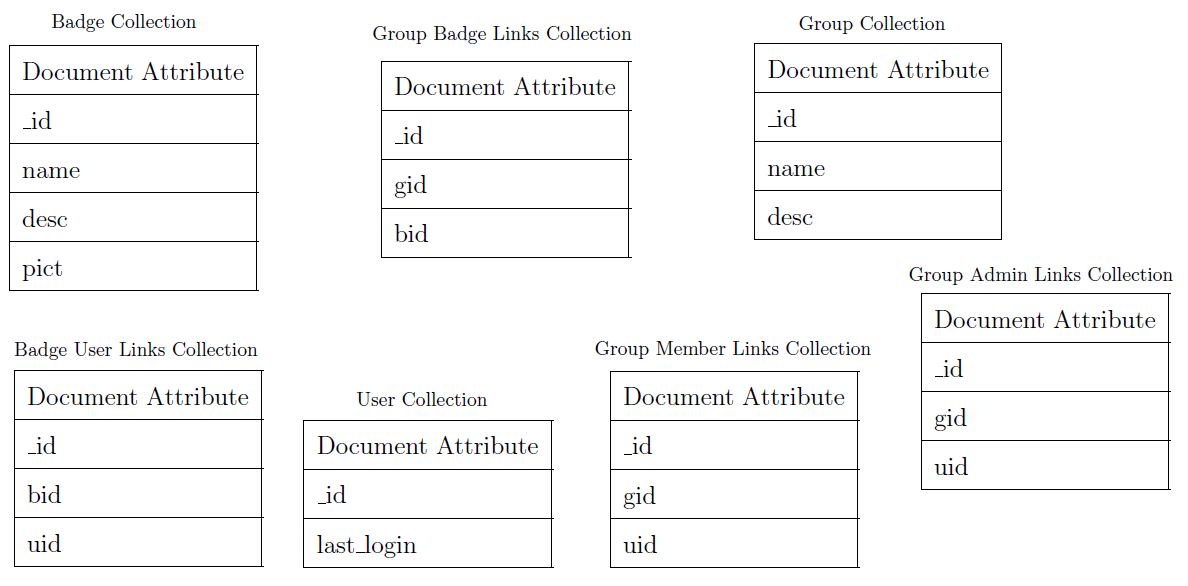
\includegraphics[height=4.1in,width=5.5in]{images/ER.png}
\caption{GradeBadge MongoDB Collections }
\label{fig:db}
\end{center}
\end{figure}

\subsection{User Collection}
The user collection contains user documents, which contain the information shown in Table~\ref{table:UserCollection}.

\begin{table}[H]
\caption{User Collection}
\vspace{-0.2in}
\textbf{ }
\begin{center}
\begin{tabular}{ | l | l |  l | }
\hline
Document Attribute & Sample Data & Description \\ \hline
{\_}id & 34728373 & Facebook user ID \\ \hline
last{\_}login & 12/1/13 12:34:56 PM & User last login timestamp   \\ \hline
\end{tabular}
\label{table:UserCollection}
\end{center}
\end{table}

\subsection{Group Collection}
This collection contains of group documents,  Table~\ref{table:GroupCollection}

\begin{table}[H]
\caption{Group Collection}\label{table:GroupCollection}
\vspace{-0.2in}
\textbf{ }
\begin{center}
\begin{tabular}{ | l | l |  l | }
\hline
Document Attribute & Sample Data & Description \\ \hline
{\_}id &  51466591b95b2b5023000001 & Auto-generated Group ID \\ \hline
name & Yoga CSUSB & Group name   \\ \hline
desc & This is Yoga group in CSUSB & Group description   \\ \hline
\end{tabular}
\end{center}
\end{table}


\subsection{Badge Collection}
The badge collection contains badge documents. Table ~\ref{table:BadgeCollection} shows the information contained in badge documents.

\begin{table}[H]
\caption{Badge Collection}\label{table:BadgeCollection}
\vspace{-0.2in}
\textbf{ }
\begin{center}
\begin{tabular}{ | l | l |  l | }
\hline
Document Attribute & Sample Data & Description \\ \hline
{\_}id & 514e34507075ae0c0f000001 & Auto-generated Badge ID \\ \hline
name & Attended 10 classes & Badge name   \\ \hline
desc & This is badge description & Badge description   \\ \hline
pict & pict1.png & Badge Picture Reference   \\ \hline
\end{tabular}
\end{center}
\end{table}


\subsection{Group Admin Links Collection}
The group-admin link collection contains documents that define the admin users of groups.  Table~\ref{table:GroupAdminLinksCollection} shows the information contained in the group-admin linking document.

\begin{table}[H]
\caption{Group Admin Links Collection}\label{table:GroupAdminLinksCollection}
\vspace{-0.2in}
\textbf{ }
\begin{center}
\begin{tabular}{ | l | l |  l | }
\hline
Document Attribute & Sample Data & Description \\ \hline
{\_}id & 514e34507075ae0c0f000001 & Auto-generated Document ID \\ \hline
gid & 514e34507075ae0c0f000123 & Group ID   \\ \hline
uid & 514e34507075ae0c0f000456 & User ID as Admin   \\ \hline
\end{tabular}
\end{center}
\end{table}

\subsection{Group Member Links Collection}
The group-member link collection contains documents that define the member users of groups. Table~\ref{table:GroupMemberLinksCollection} shows the information contained in the group-member linking document.

\begin{table}[H]
\caption{Group Member Links Collection}\label{table:GroupMemberLinksCollection}
\vspace{-0.2in}
\textbf{ }
\begin{center}
\begin{tabular}{ | l | l |  l | }
\hline
Document Attribute & Sample Data & Description \\ \hline
{\_}id & 514e34507075ae0c0f000002 & Auto-generated Document ID \\ \hline
gid & 514e34507075ae0c0f000123 & Group ID   \\ \hline
uid & 514e34507075ae0c0f000675 & User ID as Member   \\ \hline
\end{tabular}
\end{center}
\end{table}


\subsection{Badge User Links Collection}
The badge-user link collection contains documents that define the earner users of bagdes. Table~\ref{table:BadgeUserLinksCollection} shows the information contained in the badge-user linking document.

\begin{table}[H]
\caption{Badge User Links Collection}\label{table:BadgeUserLinksCollection}
\vspace{-0.2in}
\textbf{ }
\begin{center}
\begin{tabular}{ | l | l |  l | }
\hline
Document Attribute & Sample Data & Description \\ \hline
{\_}id & 514e34507075ae0c0f000005 & Auto-generated Document ID \\ \hline
bid & 514e34507075ae0c0f000975 & Badge ID   \\ \hline
uid & 514e34507075ae0c0f000456 & User ID as Earner   \\ \hline
\end{tabular}
\end{center}
\end{table}


\subsection{Group Badge Links Collection}
The group-badge link collection contains documents that define the badges of groups. Table~\ref{table:GroupBadgeLinksCollection} shows the information contained in the group-badge linking document.

\begin{table}[H]
\caption{Group Badge Links Collection}\label{table:GroupBadgeLinksCollection}
\vspace{-0.2in}
\textbf{ }
\begin{center}
\begin{tabular}{ | l | l |  l | }
\hline
Document Attribute & Sample Data & Description \\ \hline
{\_}id & 514e34507075ae0c0f000004 & Auto-generated Document ID \\ \hline
gid & 514e34507075ae0c0f000158 & Group ID   \\ \hline
bid & 514e34507075ae0c0f000953 & Badge ID    \\ \hline
\end{tabular}
\end{center}
\end{table}

